\documentclass{article}
\usepackage{latexsym, amssymb, amsmath, amsfonts, bbm, graphicx,float}
\usepackage{caption}
\DeclareCaptionLabelFormat{cont}{#1~#2\alph{ContinuedFloat}}
\captionsetup[ContinuedFloat]{labelformat=cont}
\usepackage{subcaption}
\usepackage[margin=2.5cm]{geometry}
%\usepackage{natbib}[authoryear]
%\setcitestyle{authoryear,open={((},close={))}}
\author{Jennifer Israelsson}

\begin{document}
	\title{Interim report}
	\maketitle
	
	\section{Introduction}
	In many places of the world, countries depend on agriculture for food and export. Predicting and modelling rainfall is therefore an important skill, that many researchers have attempted all over the world. Many reserachers have proposed different probability distributions, with the most common ones being: gamma, lognormal, exponential and Weibull (Shariffah et al, 2007) (Suhaila et al, 2011) (Stern et al, 1984). Instead of trying to fit the data to just one distribution(Shariffah et al, 2007) worked with a mixture of two distributions of the same type but with different parameters and a probability parameter to give the two distributions different weight. To determine the most suitable distribution function, either various goodness-of-fit tests are used or Akaike information criterion(Suhaila et al, 2011). Commonly used goodness-of-fit tests are: Kolmogorov-Smirnov, Cramer-von-Mises and Anderson-Darling. The problem with using several goodness-of-fit tests is that they might indicate different distribution fits as the most suitible one, since their scores focuses on different measures. The authors of (Shariffah et al, 2007) did not weight the importance of the tests differently, but choose to rank them after how many tests the specific distribution did better in. In both (Shariffah et al, 2007) and (Suhaila et al, 2011 )the authors concluded that the daily rainfall distriution was strongly connected to the surrounding topography. The authors of (Shariffah et al, 2007) also slit the data into moonsoon season and transition periods to see if the differents seasons followed different distributions, and concluded that it was a big difference between the stations depending on if they were on the east coast or the west coast. \\
	To model the occurence of rain, two common ideas is to use a binomial distribution with p equal to the number of wet days divided by the total number of days, or a Markov chain. With a Markov chain, one calculates the probability of having a pattern of a desired length, e.g what is the probability of having a rainy day if it has rained for the past two days. The problem with a Markov chain is that it assumes stationarity, i.e that the probabilities are the same for any time of the year. This is not true in most parts of the world due to seasonality. The authors in (Stern et al, 1984) instead lets the probabilites depend on a link function $h$ and some other function $g$, which depends on the rain occurence for the past days. This function g takes the form of a Fourier series and the number of harmonics is determined by using multiple regression techniques and stops including terms when no improvement is acheived by including another term. By using this method, they can use the full data set and let the probabilities vary over the year. To improve the fit even further, the authors split the occurence of rain into days of trace rain, defined as rain less then 2.5 mm, and rainy days.\\
	A different statistical approach is used in (Sanso et al, 1999), where the authors, instead of trying to fit a model to the data points, treat the data points as realisations of a multivariate normal distribution, with each station having a different month dependent mean. The data they are working with is measured in mm and does not classify any rain as "traces". This method tries to predict rainfall in both space and time, by letting the observation be a realisation of a model depending on both. They base their model on a truncated normal model
	\begin{equation*}
	z_{it} =
	\begin{cases}
	w^{\beta_t}_{it},& \text{if} \ w_{it}> 0 \\
	0, & \text{if} \ w_{it}  \leq 0 
	\end{cases}
	\end{equation*}
	where $z_{it}$ is the observed rainfall at station $i$ = $1,...,k$ and month $t$, $\beta_t > 0$ and $w$ is a normal random variable. By letting $w_t = (w_{1t}, ...,w_{kt})$, $w_t \sim N_k(\mu_t, \sigma^2_t\Sigma)$, i.e $w_t$ is a multivariate normal variable with mean vector $\mu_t$ and covariance matrix $\Sigma$. The authors let the mean depend on some spatial parameters and the entries of the covariance matrix is defined as $\Sigma_{ij} = \text{exp}(-\lambda d_{ij})$, where $\lambda >$ 0 and $d_{ij}$ is the distance between station i and j after they are projected onto a horizontal plane. By using a Bayesian method, they incorporate the uncertainty of the parameters into the posterior distribution. \\
	
	Ghana is a country in west Africas by the coast and shares boarder with Burkina Faso, C\^{o}te d'Ivoire and Togo. It has five distinct geographical area: low plains in the south, the Volta Basin in the centre with the artificial lake 'Lake Volta', the Akwapim-Togo ranges to the east of the Volta Basin with many heights and folded strata, the Ashanti Uplands to the west and high plains in the north (FAO, 2005). The temperature is peaking around February-March and at its lowest around August. Ghana has three distinct rainfall behvaiours. The northern part experiences an unimodal season with the rainy season between April and September, wheras the rest of the country has a bimodal season, first one in April to July and the second in September to November. The difference is that some parts of the country has two modes of the same amplitude wheras others have peaks of different amplitudes. But they all have in common a slowly increasing peak but a rapid decrease in October(Nkrumah et al, 2014). The different rain patterns depend on a few wind and pressure phenomenons. It is strongly affected by the  position of the \textbf{Inter-tropcial convergence zone}, which goes between the nothern and southern tropics every year. As ITCZ moves from the nothern position to the southern and back, the opposing prevailing winds gives rise to the West African monsoon which shows as the two rainy seasons. The rainy season in the north corresponds to when the ITCZ are at its most nothern position.The prevailing winds north of the ITCZ is called the Harmmatan and brings hot and dusty air from the Sahara desert between Dacember and March, which gives rise to the very dry season. The prevailing wind south of ITCZ is southwesterly and instead brings humid air from the Atlantic ocean.\\
	
	In this project I will start to look at if it is resonable to fit the entire data set in each month, after dividing the data into groups depending on rainfall pattern, to a single distribution or if you can get a more accurate distribution fit if only using values up to a certain value. To investigate this I will first use Quntile-Quantile ,QQ, plots to find probable threshold values and then use goodness-of-fit tests to see if there has been an improvment in the fit. 
	
	\section{Probability}
	The most commonly used distributions for daily rainfall amounts are gamma, lognormal, exponential and Weibull, eventhought the last one is an extreme value distribution. In this report, my first attempt has been to fit the data to a gamma distribution by Maximum likelihood estimation, MLE, and tried to fit the data to the other distibutions mentioned if I did not get a good fit based on QQ plots. MLE is a method of choosing parameters that maximizes the likelihood function, by differentiating the log liklihood fuction with respect to the parameter to be estimated, and then equate it to zero, we obtain the parameter. This method gives the smallest variance comapred to other parameter estimation methods such as method of moments and generalized probability weighted moments (Shariffah et al, 2007). \\
	\textbf{Gamma distribution: } The gamma distribution is a two-parameter continuous distribution family, characterized by a shape parameter, $\alpha$, and a scale parameter, $\theta$, both positive. For a random variable X the probability distribution function,PDF, mean and variance is given by,
	\begin{equation*}
	f(x ; \alpha, \theta) = \frac{x^{\alpha-1} e^{-\frac{x}{\theta}}}{\theta^\alpha \Gamma(\alpha)}, \ x > 0
	\end{equation*}
	\begin{center}
		$E(X) = \alpha\theta$, $Var[X] = \alpha\theta^2$
	\end{center}
	\textbf{Weibull: }The Weibull distribution is a two parameter distribution depending on a shape parameter $k$ and a scale parameter $\lambda$, both positive. For a random variable X the PDF, mean and variance is given by,
	\begin{equation*}
	f(x ; k, \lambda) = \frac{k}{\lambda}\left(\frac{x}{\lambda}\right)^{k-1}e^{(-x/ \lambda)^k}, \ x> 0
	\end{equation*}
	\begin{equation*}
	E(X) = \lambda\Gamma\left(1+\frac{1}{k}\right), \ Var[X] = \lambda^2\left[\Gamma\left(1 + \frac{2}{k}\right)- \left(\Gamma\left(1 + \frac{1}{k}\right)\right)^2\right]
	\end{equation*}
	\subsection{Statistical test}
	To compare different fitted distributions and determine the most suitible ones, one can use both statistical and graphical methods. Graphical methods, such as QQ plots, offers a fast way of comparing your data to a fitted model or looking at general behaviour of the data, wheras statistical tools quantifies how similar two distributions are two each other by calculating various measures of distance such as maximum distance between distribution functions. The issue with applying goodness-of-fit tests to large data sets is that your p-values can be very small, hence suggest you to reject your null hypothesis, when in reality the difference is very small. It is therfore difficult to use these test to determine if the fitted model is suitable, but can be used to compare the fit of two different models if they have a similar size on their data sets.
	
	\subsubsection{Statistical tools}
	\textbf{Wilcoxon signed rank test:} Is a non-parametric test that either tests the null hypothesis that a sample has a certain median or the null hypothesis that two paired samples comes from the same distribution. In the paired case, you take the difference between each pair, rank the difference from smallest to largest absolut value and then add up all the ranks of the positive differences. If this value is greater then the table value for our number of pairs, we reject the null hypothesis and conclude that the data comes from different distributions. 
	 This test can be used to test if the median in months has significantly changed over a time period, given that they have he same pattern. If we compare two sets, one sample with the peak in April and one sample with the peak in September, they will clearly behave differently but the test will give the same weight to the positive and the negative rankings, so we will not reject our null hypothesis. \linebreak
	\textbf{Kolmogorov-Smirnov test:} This test is used to test if our emperical cumulative distribution function and our assumed theoretical one are close enough. The test statistic is given by,
	\begin{equation*}
	D_n = sup_x |F_n(x) - F(x)|
	\end{equation*}
	where $F_n$ is our empirical distrbution function, EDF, and $F$ is the cumulative distribution function, CDF, that we are testing against. We reject our null hypothesis if $D_n$ is larger then our table value.\\
	\textbf{Anderson-Darling test:} Both this test and the Cram\'{e}r-von Mises test belongs to the class of quadratic EDF statistics, where this test puts bigger weight on the tail behaviour. The test statistics, A, of our ordered data ${x_1, x_2, ..., x_n}$, is defined as,
	\begin{equation*}
	A^2 = -n - S
	\end{equation*}
	where
	\begin{equation*}
	S = \sum_{i=1}^n\frac{2i -1}{n}[\text{ln}(F(x_i)) + \text{ln}(1 - F(x_{n+1-i}) )]
	\end{equation*}
	where $F$ is the CDF that we are testing our data against. \\
	\textbf{Cram\'{e}r-von Mises:} This test is similar to the Anderson-Darling test. We once again test our increasingly ordered data ${x_1, x_2,...,x_n}$ with a CDF $F$ with the test statistic,
	\begin{equation*}
	T = \frac{1}{12n} + \sum_{i=1}^{n}\left[\frac{2i-1}{2n} - F(x_i)\right]^2
	\end{equation*}
	and reject our null hypothesis if the T value is larger then the table value.\\
	\textbf{Akaike information criterion:} Is an estimator of how good a model is compared to other models, fitted to the same data set. The number does not tell if the model is a good fit or not, only if it is a better fit then some other model. The best model fit is the one with the lowest value. 
	\subsubsection{Graphical methods}
	\textbf{Quantile-Quantile plots, QQ}: A QQ  plot compares the quantiles of our data, with the qunatiles of our assumed distribution. If these two distributions agree, our data will fall on an approxiamatly straight line. If our data falls below the straight line, our assumed distribution is more heavy tailed then our data, meaning that our data has fewer higher values then expected. If our data insteads falls above the straight line, our assumed distribution is too light tailed. \\
	\textbf{Autocorrelation plot:} Autocorrelation describes how correlated the time series data is to itself, i.e how dependent is the data a few days forward on the day today. By plotting correlation as a function on number of lag days, we can see roughly how long a wet spell is in each month. For autocorrelation to work, there can be no missing values, so one needs to remove the months from the data with missing values. 
	\subsection{Extreme value theory}
	\subsubsection{Maximum analysis}
	In extreme value theory, we only look at the larger values in our data instead of all the data, to get a better understanding of how the tail behaves, and gives us a more accurate way to extrapolate outside our data. We divide our data into suitible blocks, e.g years or months, and denote $M_n$ = max$(X_1,...,X_n)$, i.e the maximum value of our n sample points in each block. This is often called a block maxima. We are interested in finding the distribution of $M_n$ as n increases. We call a non-degenerated rv X \textit{max-stable} if
	\begin{equation*}
	c_nX + d_n = M_n
	\end{equation*}
	for all n $\geq$ 2 and appropriate $c_n>0$, $d_n \in \mathbb{R}$. Under the assumption that all our $X_i$'s are independent and identically distributed, we also have that
	\begin{equation*}
	\mathbb{P}(M_n \leq x) = \mathbb{P}(X_1 \leq x,...,X_n \leq x) = F^n(x)
	\end{equation*}
	with F being the distribution function of the rv X. This leads us to the important \textit{Fisher-Tippet theorem}, which states that; if there exists norming constants $c_n$ and $d_n$ as above and some non-degenerated distribution function H such that
	\begin{equation}
	c_n^{-1}(M_n - d_n) \xrightarrow{d} H
	\end{equation}
	then H belongs to one of the three extreme value distributions; Fr\'{e}chet, Gumbel or Weibull. These can be summarised in one distribution, called \textit{Generalised extreme value} distribution, GEV. 
	\begin{equation*}
	H_\xi(x) = 
	\begin{cases}
	\text{exp}(-(1+\xi x)^{-1/\xi}), & \text{if} \ \xi \neq 0 \\
	\text{exp}(-(\text{exp}(-x))), & \text{if} \ \xi = 0 
	\end{cases}
	\end{equation*}
	where $1+\xi x > 0$. With $\xi = 0$, we get Gumbel, $\xi > 0$ Fr\'{e}chet and $\xi < 0$ Weibull. Closely related to GEV distributions is \textit{maximum domain of attraction}. We say that a rv X belongs to the \textit{maximum domain of attraction} of \textit{H}, X $\in MDA(H)$, if there exists norming constants $c_n$ $>$ 0, $d_n \in \mathbb{R}$ such that (1) holds.

	\subsubsection{Upper order analysis}
	Instead of looking at maxima, and thereby throwing away a lot of data, we can look at all values above a threshold, u. We can look at both the distribution and the mean of the data above this threshold
	\begin{equation*}
	F_u(x) = \mathbb{P}(X - u \leq x | X > u) = \frac{F(x + u) - F(u)}{1 - F(u)}
	\end{equation*}
	\begin{equation*}
	e(u) = \mathbb{E}(X - u | X > u)
	\end{equation*}
	$e(u)$ is called \textit{the mean excess function of X}. Just like the block maxima converges to a GEV distribution, the data over a high threshold also converges to a distribution, called the \textit{General pareto distribution}, GPD
	\begin{equation*}
	G_{\xi, \nu, \sigma}(x) =
	\begin{cases}
	1-(1+\xi \frac{x-\nu}{\sigma})^{-1/\xi}, & \text{if} \ 1+\xi \frac{x-\nu}{\sigma} > 0, \xi \neq 0 \\
	1- e^{-\frac{x-\nu}{\sigma}}, & \text{if} \  \xi = 0
	\end{cases}
	\end{equation*}
	where
	\begin{equation*}
	\begin{cases}
	x \geq 0, & \text{if} \ \xi \geq 0 \\
	0 \leq x \leq -\sigma/ \xi, & \text{if} \ \xi < 0
	\end{cases}
	\end{equation*}
	$\nu \in \mathbb{R}$ is called a location parameter and $\sigma>0$ is a scale parameter. The two distributions are related, such that the distributions for which the block maxima converges to a GEV with parameter $\xi$, their excess distribution converges to the GPD with same shape parameter $\xi$. 
	
	\section{Data}
	The data that will be used in this report is 30 years of daily precipitation data from 21 stations around Ghana. A overview of the data is displayed in table \ref{Tstations}. Because of many missing values, the stations BEK, ABE and AKA has been excluded from further analysis, and station NAV and WA has been excluded because their data sets are close to identical to TLE.
	\subsection{Overall data structure}
	
	\begin{table}[H]
		\centering
		\begin{tabular}{| c | c | c | c | c| c| c | c | c |}
			\hline
			Station & Long. & Lat. & Pos. Obs. & Missing obs. & Days (Dec, Jan, Feb) & Annual mean & Rainy day mean & Mode \\
			\hline
			AXM & -2.23 & 4.86 & 4282 & 58 & 214, 104, 154 & 1874 & 13.13 &  Semi-bi \\
			ODA & -0.98 & 5.93 & 4180 & 0 & 140, 60, 151 & 1407 & 10.10 & Bi \\
			BEK & -2.33 & 6.2 & 3851 & 366 & 80, 6, 141 & 1394 & 10.50 & \\
			KDA & -0.25 & 6.08 & 3756 & 30 & 112 , 81, 167 & 1293 & 10.33 & Bi\\
			ABE & -0.73 & 6.65 & 3415 & 700& 65, 46, 112 &1277 & 10.47 &  \\
			KSI & -1.6 & 6.71 & 3586 & 0 & 80 , 51, 136 & 1347 & 11.27 & Bi \\
			HO & 0.46 & 6.6 & 3409 & 0& 86, 52, 140 & 1276 & 11.23& Bi \\
			TDI & -1.76 & 4.88 & 3312 & 28 & 113, 37, 92 & 1079 & 9.77 & Semi-bi\\
			SUN & -2.33 & 7.33 & 3187 & 61 & 52, 23, 106 & 1191 & 11.22 & Bi\\
			WEN & -2.1 & 7.75 & 3188 & 2& 48, 24, 90 & 1249 & 11.75& Bi \\
			KRA & -0.03 & 7.81 & 2991 & 0 & 30, 20, 35 & 1366 & 13.70 & Uni\\
			BOL & -2.48 & 9.03 & 2688 & 2 &  21, 7, 29 & 1101 & 12.29 & Uni\\
			SAL & -1.06 & 5.2 & 2679 & 123 & 52, 23, 106 & 931 & 10.43 & Semi-bi\\
			NAV & -0.01 & 9.45 & 2623 & 62& 6, 6, 22 & 1024 & 11.71 & \\
			WA & -2.5 & 10.1 & 2609 & 62 & 6, 6, 22 & 1018 & 11.70 &  \\
			TLE & -0.85 & 8.5 & 2599 & 31 & 7, 6, 23 & 1017 & 11.74 & Uni\\
			AKA & 0.8 & 6.11 & 2236 & 580 & 74, 23, 56 & 848 & 10.99 & \\
			NAV1 & -1.1 & 10.9 & 2184 & 32 & 4, 2, 11 & 988 & 13.57 & Uni\\
			ACC & -0.16 & 5.6 & 2130 & 6 & 54, 29, 56 & 747 & 10.52 & Semi-bi \\
			ADA & 0.63 & 5.78 & 2037 & 0 & 37, 21, 58 & 790 & 11.63 & Semi-bi\\
			TEM & 0 & 5.61 & 1840 & 31 & 42, 23, 49 & 659 & 10.75 & Semi-bi \\
			\hline
		\end{tabular}
		\caption{All stations}
		\label{Tstations}
	\end{table}

	By plotting the monthly average of each station, one can easily see a clear uni-, bi- and semibimodal behaviour for each station. I have therefore grouped the stations into these three categories and plot these 3 groups monthly averages instead, to get even more data to work with (fig \ref{MonAvegroups}). Plotting the stations on a map, colour coded by their rainmode (fig \ref{mapRainmode}), one can clearly see the pattern of only one rainy season in the north and two in the south, with a stronger rainy season in April for the coast station and two even rainy seasons for the central stations. This confirms the pattern that others have observed and explained with the shift in the ITCZ.\\
	If we compare the two monthly average plots for the unimodal stations, we can see that the extreme values ($\geq$ 150mm, 40 observations), has an impact on the spread in the rainiest months, but does not affect the overall pattern of the means. But it has a rather big impact on the distribution within the rainier months, especially August and September that goes from being normally distributed to being right skewed, i.e the larger half of the values have a bigger spread then the lower half. The number of outliers are also reduced by removing the extreme values. Other than that, the two plots looks very much the same, with the dry season months staying the exact same, which is to be expected.
	The semibimodal stations are less effected by removing the higher values, probably because we have so many more large observations in these stations that can compensate for a few very large values. The very obviouse difference is in June, since it becomes much more compact by removing it, but it still has one outlier. Just like for the unimodal stations, most of the outliers disappear when removing the extremes and the dry season stays invariant. The semibi stations are more normally distributed then the unimodal but about the same spread in the rainy seasons. A similar thing is observed with the bimodal stations, but we still have quite a few outliers even after removing the extremes. Only June has changed its maximum value, so removing extremes seems to make the least difference in this group. 
	\begin{figure}[H]
		\centering
		\begin{subfigure}{0.5\textwidth}
			\centering
			\includegraphics[width=1\linewidth]{MonAveUni.pdf}
			\caption{Unimodal}
		\end{subfigure}%
		\begin{subfigure}{0.5\textwidth}
			\centering
			\includegraphics[width=1\linewidth]{MonAveUniN.pdf}
			\caption{Unimodal, capped}
		\end{subfigure}
		\begin{subfigure}{0.5\textwidth}
			\centering
			\includegraphics[width=1\linewidth]{MonAveBi.pdf}
			\caption{Bimodal}
		\end{subfigure}%
		\begin{subfigure}{0.5\textwidth}
			\centering
			\includegraphics[width=1\linewidth]{MonAveBiN.pdf}
			\caption{Bimodal, capped}
		\end{subfigure}
		\begin{subfigure}{0.5\textwidth}
			\centering
			\includegraphics[width=1\linewidth]{MonAveSemi.pdf}
			\caption{Semi-bimodal}
		\end{subfigure}%
		\begin{subfigure}{0.5\textwidth}
			\centering
			\includegraphics[width=1\linewidth]{MonAveSemiN.pdf}
			\caption{Semi bi modal, capped}
		\end{subfigure}
		\caption{Monthly averages for each rain mode group}
		\label{MonAvegroups}
	\end{figure}

\begin{table}
	\centering
	\begin{tabular}{|c|c|c|c|c|c|c|c|c|}
\hline
\textbf{Uni} &mean &  sd& median &mad & min &  max& skew &kurtosis \\
\hline
jan  &  2.28 & 3.15 &  0.64 & 0.8 &0.02 &10.62 & 1.28 & 0.17 \\
\hline
feb  &  5.07& 5.35 &  3.12 & 3.77 &0.28 &21.43& 1.47&1.57 \\
\hline
mar  &  18.63 &8.41  &17.27 & 8.81 &5.57 &35.48& 0.23 &-0.89 \\
\hline
apr & 56.23& 13.34&  55.08  & 12.22& 29.43& 84.48 &0.21 & -0.66 \\
\hline
may  & 80.83& 16.45 &  80.72 &20.4 &44.3 &117.93 &0.04 & -0.56 \\
\hline
jun &109.71 &18.02& 107.38 &16.95 &77.48 &148.87&0.31  &-0.62 \\
\hline
jul & 114.86 &18.59 &113.22 &21.4 &87.92 &178 &  1.1 & 2.05 \\
\hline
aug &146.66& 34.63& 142.12 & 41.53& 98.38 &238.3 & 0.65  &-0.27 \\
\hline
sep &136.47& 19.23 &135.26 & 16.86 &95.57 &193.25&  0.41 &0.95 \\
\hline
oct &63.9& 15.22  &61.93 & 16.63& 33.47 &89.05& 0.06& -1.05  \\
\hline
nov &7.89 &5.2  & 6.43  & 3.25& 1.58 &20.52 &0.97 & -0.19 \\
\hline
dec& 3.04& 3.32 &  1.79  &  2.14 & 0.12& 13.38& 1.37 & 1.26 \\
\hline
\textbf{Bi} & & & & & & & & \\
\hline
jan &16.66 &6.54  & 15.6 &5.99 &4.72& 30.12& 0.26& -0.75 \\
\hline
feb  &47.25 &12.85 & 45.14 & 10.82 &23.75 &73.97&0.25 & -0.69 \\
\hline
mar &105.9 &12.98 &107.71  &11.63 &80.27& 129.5& -0.23 & -0.75 \\
\hline
apr &150.31 &18.14& 153.32 & 21.98 &117.82 &182.5 & -0.13 &-1.24 \\
\hline
may &158.76 &22.73 &158.79  &26.63 &118.87 &215.94& 0.23 &-0.23 \\
\hline
jun &188.5 &28.26 &178.88  &33.11 &147.43& 243.17 & 0.24  &-1.34 \\
\hline
jul &125.28 &26.56& 122.78 & 25.71 &83.07& 216.83 &1.19  &2.4 \\
\hline
aug &84.85 &10.92 & 85.61 &10.4 &65.28 &112.2 & 0.42 & -0.18 \\
\hline
sep &159.07& 23.79& 156.04 & 23.04 &117.25 &204.13&0.18 &-0.74 \\
\hline
oct &166.45 &17.04 &170.68  &12.21 &118.48& 196.97&-0.97 &0.89 \\
\hline
nov &62.91& 9.4 & 65.62 & 10.09 &43.55& 74.6 & -0.59& -0.92 \\
\hline
dec  &27.49 &8.21 & 27.99 & 5.16 &10.72 &52.8 &0.57 & 1.25 \\
\hline
\textbf{Semi} &  & & & & & & & \\
\hline
jan &14.71 &6.52 & 12.96 & 5.98 &5.25 &33.18& 0.93& 0.26 \\
\hline
feb &26.87 &9.73  &25.78 & 9.64 &8.12& 55.95 &0.63 & 0.74 \\
\hline
mar &61.51 &17.47 & 56.95&11.18 &35.93& 106.37 &1.04 & 0.32 \\
\hline
apr &106.34 &23.21& 103.82 & 26.96 &75.67& 162.97& 0.57 & -0.55 \\
\hline
may &181.48&26.85& 177.67 &27.71 &128.53& 249.35& 0.4 &-0.1 \\
\hline
jun &236.12 &37.12 &233.34 &34.51 &162.9& 327.5 & 0.33 & -0.13 \\
\hline
jul &78.95& 17.02 &  75.7 & 18.85& 51.75 &125.97 & 0.52& 0 \\
\hline
aug& 33.73& 8.4  &32.94 &6.3 &15.35 &50.88 & 0.08 & -0.3 \\
\hline
sep &59.62 &16.86 & 54.84 & 14.22 &35.63 &93.1 &0.53 & -0.94 \\
\hline
oct &106.59& 18.01 &109.67 & 22.68 &70.1 &135.75 &-0.19  &-1 \\
\hline
nov &55.45 &13.01 & 54.47 & 14.84 &32.93 &82.85 &0.25 & -1.03 \\
\hline
dec &28.64 &11.52 & 26.88 & 11.48 &14.2 &69.45& 1.43 & 2.85 \\
\hline
\end{tabular}
\caption{Descriptive data, monthly average}
\label{MonAveTab}
\end{table}

		\begin{figure}
			\centering
			\includegraphics[width=0.4\linewidth]{mapRainmode.pdf}
			\caption{Rain modes}
			\label{mapRainmode}
		\end{figure}
		\begin{figure}[H]
		\centering
		\begin{subfigure}{0.4\linewidth}
			\centering
			\includegraphics[width=1\linewidth]{mapObs.pdf}
			\caption{Positive observations in \%}
		\end{subfigure}%
		\begin{subfigure}{0.4\linewidth}
			\centering
			\includegraphics[width=1\linewidth]{mapObsnorm.pdf}
			\caption{Positive observation in \%, $>$ 1mm}
		\end{subfigure}
		\begin{subfigure}{0.4\linewidth}
			\centering
			\includegraphics[width=1\linewidth]{mapAnMeannorm.pdf}
			\caption{Annual mean, $>$ 1mm}
		\end{subfigure}%
		\begin{subfigure}{0.4\linewidth}
			\centering
			\includegraphics[width=1\linewidth]{mapDayMeannorm.pdf}
			\caption{Daily mean on rainy days, $>$ 1mm}
		\end{subfigure}
		\caption{Observations, annual mean, daily mean}
		\label{maps}
	\end{figure}
	Looking at the values in table \ref{MonAvegroups}, we can see that the mean and the median is very close to each other for all stations and months. The \textit{mean absolute deviation} varies a lot between months within groups and between groups, where we for example have a very low value for August in Semi but very large in Uni, which is to be expected since we have a larger spread in rainy months than dryer. We can once again see the big difference in the dryer months between the north and the other stations, with the north having a much dryer Dec-Feb then the other. Disscusion on appropriate values for the skew and kurtosis range for data to be normally distributed varies from 0.8 up to 3, with many stating 2 to be the general value. If we use 2, all months are considered to be normally symmetrical distributed but if we use 0.8 , the dry period in the north and Semi and the most extreme months in Bi is not. Nearly all months in Bi is having a negative kurtosis wheras for the other only half are negative. So many of the sets are more lightly tailed then a normal distribution.\\
	
	We can see that the number of positive observations varies a lot, with most observations in the midlands and the station "AXM", and fewer in the north and along rest of the coastline. We get nearly the exact same distribution whether we include rain amounts less then 1 mm or not. The annual mean is close to identical if we discard all observations $<$ 1mm, sometimes refered to as trace values, which makes sense since they are very small and will not have that much of an impact on an annual scale. But if we look at the rainy day mean, we see, as expected, an increase in the mean, but also a slightly different distribution. If we include all positive values, we have a very low mean on the station "TDI" and relatively high means in the north. But if we discard the trace values, we see a higher mean compared to the other stations along the coast and a lower mean in comparison with other stations in the north. This tells us that we have many extremly small values along the coast, but much less in the north and the midlands, which could be because of higher humidity by the ocean.
	
	In fig \ref{MaxAll} we can see the maximum value in each month and station. This shows that some months have a big spread and others are much closer together. We can see that the values in January and December are clustered together, except from station "NAV1" (dashed violet line) which is much lower and station "KSI" (dashed gray) in January which is much higher and "BEK" (solid blue) and "KSI" in December which both are larger. It is also clear that the spread in April and September is much smaller, and February is even closer if we ignore "NAV1". So we have a smaller spread in maximum rainfall during the rainiest months than we do in the dry season in general and a very big spread in the two transition months (March, October).
	
	\begin{figure}[H]
		\centering
		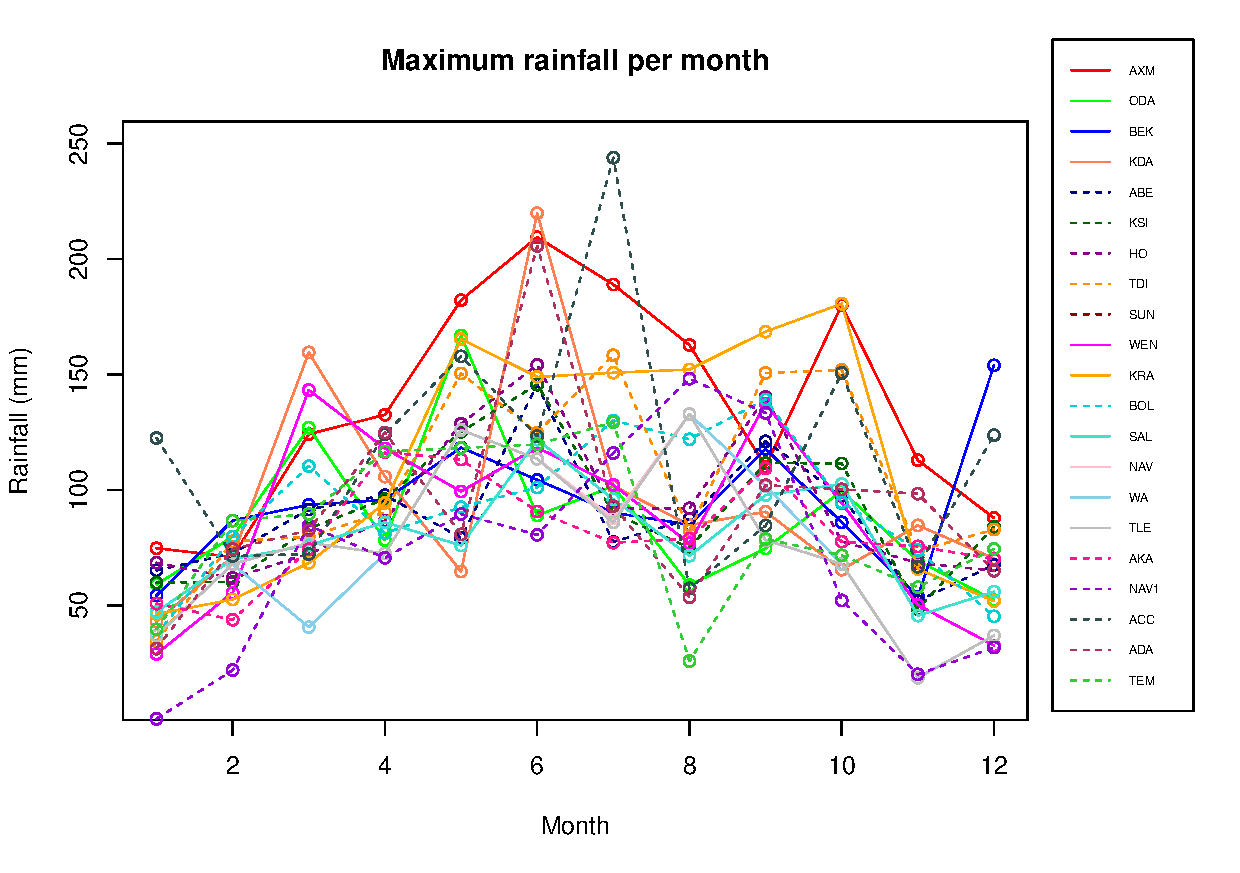
\includegraphics[width=1\linewidth]{MonMax.pdf}
		\caption{Maximum value in each month, all stations}
		\label{MaxAll}
	\end{figure}
	
	\section{Results}
	\subsection{Distribution fit}
	Because of sesonal rain behaviour, a dry period in December-February and one or two rainy seasons in April-July and September-October, each month has been considered seperatly. To also account for the different rain seasons, I have keept the three groups introduced in the previous section. By keeping the stations in groups instead of analysing each station one by one, we get a bigger data set to work with, but also automatically introduce more variation since the stations are not having identical behaviours, as seen in table \ref{Tstations} and \ref{maps}. I have decided to exclude December-February in the unimodal group because of too few data points. For all other months in all groups, I have tried and fit the data to a gamma distribution by MLE. I have thereafter plotted a histogram with the estimated denisty function, a QQ plot, the empirical and theoretical cumulitative density function and a Probability-Probability plot, to get a graphical idea if it is a resonable fit or not. In cases where the gamma distribution has not been a good fit, I have instead tried to fit the data to a lognormal, exponential and Weibull distribution. If all of them look equally good, I picked the distibution with the lowest AIC. For distribution fits where the QQ plot looks straight up to a certain value and then wonders of in some direction, I have fitted a new gamma distribution to only the values lower then that value to see if I could get a better graphical fit. If the QQ plot looked better after refitting the data, I used the goodness-of-fit tests Kolmogorov-Smirnov, Anderson-Darling and Cramer-von-Misen, to test if they are in fact better fits. 
	\subsubsection{Unimodal stations (KRA, BOL, TLE, NAV1)}
	As many other has discovered, the rain distribution in the north only has one rainy season, which clearly can be seen in fig \ref{MonAvegroups}. The only missing data points in this group is from one full November and one full December and it has got proportionaly equally many positiv observations as the semi-bimodal group, but very differently distributed. By looking at QQ plots of the months (fig \ref{GammaFitUni}), we can see that June and August fits perfectly well to their distributions, and May only has a couple of observations that does not fit. But April, July, September and October fits poorly after 80 mm and March after 60 mm. November is a poor fit in general, but that most likely depends on the lack of data and can therefore not be improved. 
	\begin{figure}[H]
		\ContinuedFloat*
		\centering
		\begin{subfigure}{0.5\textwidth}
			\centering
			\includegraphics[width=1\linewidth]{UniFitMar.jpg}
			\caption{March,(15.633, 0.633) }
		\end{subfigure}%
		\begin{subfigure}{0.5\textwidth}
			\centering
			\includegraphics[width=1\linewidth]{UniFitApr.jpg}
			\caption{April, (19.673, 0.674)}
		\end{subfigure}
		\caption{Gamma distribution fits, Unimodal group}
		\label{GammaFitUni}
	\end{figure}
	\begin{figure}[H]
		\ContinuedFloat
		\centering
		\begin{subfigure}{0.5\textwidth}
			\centering
			\includegraphics[width=1\linewidth]{UniFitMay.jpg}
			\caption{May, (18.326, 0.705)}
		\end{subfigure}%
		\begin{subfigure}{0.5\textwidth}
			\centering
			\includegraphics[width=1\linewidth]{UniFitJun.jpg}
			\caption{June, (19.902, 0.703) }
		\end{subfigure}
		\begin{subfigure}{0.5\textwidth}
			\centering
			\includegraphics[width=1\linewidth]{UniFitJul.jpg}
			\caption{July, (19.678, 0.663)}
		\end{subfigure}%
		\begin{subfigure}{0.5\textwidth}
			\centering
			\includegraphics[width=1\linewidth]{UniFitAug.jpg}
			\caption{August, (22.687, 0.614)}
		\end{subfigure}
		\begin{subfigure}{0.5\textwidth}
			\centering
			\includegraphics[width=1\linewidth]{UniFitSep.jpg}
			\caption{September, (17.848, 0.716)}
		\end{subfigure}%
		\begin{subfigure}{0.5\textwidth}
			\centering
			\includegraphics[width=1\linewidth]{UniFitOct.jpg}
			\caption{October, (15.229, 0.726)}
		\end{subfigure}
		\caption{Gamma distribution fits, unimodal group}
	\end{figure}
	To try and improve the fit, one can cut of all values larger than where they start to wander off and fit a seperate extreme distribution to the higher values. By trying different splitting values, it was possible to improve the fit, at least graphically, for all months except April (fig \ref{UniCap}). But when tested with the three mentioned goodness-of-fit tests, it showed that only some of the months got a better fit with the capped data set. Both October and March got much higher p-values (March: KS 6\% to 10\%, CVM 3\% to 6\%, October: KS 4\% to 6\%, CVM 3\% to 4\%) with the capped data sets with all the tests, April and July showed no improvment and September even performed worse. The biggest change in the scale value is seen in March, which could potentially be since it is the transition month into the rainy season, but the scale value changed a lot less for October, which is the other transition month. 
	\begin{figure}[H]
		\centering
		\begin{subfigure}{0.4\textwidth}
			\centering
			\includegraphics[width=1\linewidth]{UniFitMar70.jpg}
			\caption{March, Data $<$ 70, (12.805, 0.681)}
		\end{subfigure}%
		\begin{subfigure}{0.4\textwidth}
			\centering
			\includegraphics[width=1\linewidth]{UniFitJul120.jpg}
			\caption{July, Data $<$ 120, (18.668, 0.677)}
		\end{subfigure}
			\begin{subfigure}{0.4\textwidth}
			\centering
			\includegraphics[width=1\linewidth]{UniFitSep100.jpg}
			\caption{September, Data $<$ 100, (16.5, 0.74)}
		\end{subfigure}%
			\begin{subfigure}{0.4\textwidth}
			\centering
			\includegraphics[width=1\linewidth]{UniFitOct100.jpg}
			\caption{October, Data $<$ 100, (14.433, 0.744)}
		\end{subfigure}
		\caption{Gamma fits with capped data}
		\label{UniCap}
	\end{figure}	
	\subsubsection{Bimodal stations (ODA, KDA, KSI, HO, SUN, WEN)}
	For these stations, we see a very similar pattern in the montly distributions as for the unimodal group. Just like there, we have that March is right skewed i.e the data has more large values then expected from the fitted distribution and April left skewed i.e less large values then expected, May is a good fit except for the few largest values and September gets a poorer fit after 70 mm. But here June and August are much more left skewed then for the unimodal stations and July appears not to be gamma distributed at all. The dry season months show a nearly perfect fit. 
		\begin{figure}[H]
		\ContinuedFloat*
		\centering
		\begin{subfigure}{0.4\textwidth}
			\centering
			\includegraphics[width=1\linewidth]{BiFitJan.pdf}
			\caption{January, (15.983, 0.648)}
		\end{subfigure}%
		\begin{subfigure}{0.4\textwidth}
			\centering
			\includegraphics[width=1\linewidth]{BiFitFeb.pdf}
			\caption{February, (15.275, 0.705)}
		\end{subfigure}
		\caption{Gamma distribution fits, bimodal group}
		\label{GammaFitBi}
	\end{figure}
		\begin{figure}[H]
		\ContinuedFloat
		\centering
		\begin{subfigure}{0.5\textwidth}
			\centering
			\includegraphics[width=1\linewidth]{BiFitMar.pdf}
			\caption{March,(18.644, 0.666)}
		\end{subfigure}%
		\begin{subfigure}{0.5\textwidth}
			\centering
			\includegraphics[width=1\linewidth]{BiFitApr.pdf}
			\caption{April, (19.447, 0.737)}
		\end{subfigure}
		\begin{subfigure}{0.5\textwidth}
			\centering
			\includegraphics[width=1\linewidth]{BiFitMay.pdf}
			\caption{May, (18.246, 0.691)}
		\end{subfigure}%
		\begin{subfigure}{0.5\textwidth}
			\centering
			\includegraphics[width=1\linewidth]{BiFitJun.pdf}
			\caption{June, (20.498, 0.627)}
		\end{subfigure}
		\begin{subfigure}{0.5\textwidth}
			\centering
			\includegraphics[width=1\linewidth]{BiFitJul.pdf}
			\caption{July, (19.122, 0.532)}
		\end{subfigure}%
		\begin{subfigure}{0.5\textwidth}
			\centering
			\includegraphics[width=1\linewidth]{BiFitAug.pdf}
			\caption{August, (13.068, 0.547)}
		\end{subfigure}
		\caption{Gamma distribution fits, bimodal group}
	\end{figure}
	\begin{figure}[H]
		\ContinuedFloat
		\centering
		\begin{subfigure}{0.5\textwidth}
			\centering
			\includegraphics[width=1\linewidth]{BiFitSep.pdf}
			\caption{September, (16.732, 0.625)}
		\end{subfigure}%
		\begin{subfigure}{0.5\textwidth}
			\centering
			\includegraphics[width=1\linewidth]{BiFitOct.pdf}
			\caption{October, (14.17, 0.73)}
		\end{subfigure}
		\begin{subfigure}{0.5\textwidth}
			\includegraphics[width=1\linewidth]{BiFitNov.pdf}
			\caption{November, (11.099, 0.736)}
		\end{subfigure}%
		\begin{subfigure}{0.5\textwidth}
			\includegraphics[width=1\linewidth]{BiFitDec.pdf}
			\caption{December, (14.223, 0.672)}
		\end{subfigure}
		\caption{Gamma distribution fits, bimodal group}
	\end{figure}
	Since July and August are so skewed, I tried to fit them to some other distributions and found that they fitted much better to a Weibull distribution. Fot the other ones, I kept the gamma distribution and only changed the splitting value. Once again, all of the months graphically improves a lot by this method but only a few get larger p-values in the goodness-of-fit tests. July and August improves greatly (July: CVM $3.1e^{-12}$ to $6.1e^{-7}$, KS 0 to $5.8e^{-9}$, August: CVM $2.2e^{-11}$ to $2.3e^{-8}$, KS 0 to $4.8e^{-12}$) by fitting them to a Weibull distribution instead of a gamma, June and September improves slightly (CVM: June $1.56e^{-5}$ to $1.77e^{-5}$, September $3.8e^{-7}$ to $7e^{-7}$) by adding the cap, but October shows no improvment and March performs worse. So here we see an improvment in the rainy months and no improvment in the transition months, right opposite to results for the unimodal stations.
	\begin{figure}[H]
		\ContinuedFloat*
		\centering
		\begin{subfigure}{0.5\textwidth}
			\centering
			\includegraphics[width=1\linewidth]{FitBiMar80.pdf}
			\caption{March, Data $<$ 80, (17.446, 0.683)}
		\end{subfigure}%
		\begin{subfigure}{0.5\textwidth}
			\centering
			\includegraphics[width=1\linewidth]{FitBiJun150.pdf}
			\caption{June, Data $<$ 150, (20.145, 0.631)}
		\end{subfigure}
	\caption{Distribution fits with capped data}
	\label{BiCap}
	\end{figure}
	\begin{figure}[H]
		\ContinuedFloat
		\centering
		\begin{subfigure}{0.5\textwidth}
			\centering
			\includegraphics[width=1\linewidth]{FitBiJulWei.pdf}
			\caption{July, Weibull distribution, (6.976 0.661)}
			\end{subfigure}%
		\begin{subfigure}{0.5\textwidth}
			\centering
			\includegraphics[width=1\linewidth]{FitBiAugWei.pdf}
			\caption{August, Weibull distribution, (5.014, 0.666)}
		\end{subfigure}
		\begin{subfigure}{0.5\textwidth}
			\centering
			\includegraphics[width=1\linewidth]{FitBiSep90.pdf}
			\caption{September, Data $<$ 90, (15.73, 0.64)}
		\end{subfigure}%
		\begin{subfigure}{0.5\textwidth}
			\centering
			\includegraphics[width=1\linewidth]{FitBiOct90.pdf}
			\caption{October, Data $<$ 90, (13.658, 0.741)}
		\end{subfigure}
		\caption{Distribution fits with capped data}
		\end{figure}
	
	\subsection{Semi-bimodal stations (AXM, TDI, SAL, ACC, ADA, TEM)}
	These stations do not seem to come from a gamma distribution since I get a poor fit for nearly all months except March and December, if we discard the largest value. January, February, May, June and November are well fitted for most of the values, but July, August, September and October diverges from the straight line very quickly. So it seems like the dry season fits much better then the rainy season.
	As I put a cap on June data, it became clearer that the lower part was very left skewed, i.e that the data contains many more points in the mid range then the fitted distribution, and that the data fitted better to a Weibull distribution, eventhough it is far from optimal. Regardless of distribution and cap, I see no improvment in the distribution fit on July or August. One possible way to deal with this is to divide the data into low, moderate and heavy rainfall, and fit different distributions to each set. The general behaviour of the months is that we have fewer observations in the low-mid range than expected and more higher values than expected. We can improve the graphical fit in January, February, April and May by capping the maximum value and June by fitting it to a Weibull distribution instead. But the other months has the pattern described above and does therfore not become any better by just adding caps or changing to a Weibull or lognormal distribution.
	
	\begin{figure}[H]
		\ContinuedFloat*
		\centering
		\begin{subfigure}{0.5\textwidth}
			\centering
			\includegraphics[width=1\linewidth]{SemiFitJan.pdf}
			\caption{January, (15.346, 0.599)}
		\end{subfigure}%
		\begin{subfigure}{0.5\textwidth}
			\centering
			\includegraphics[width=1\linewidth]{SemiFitFeb.pdf}
			\caption{February, (17.008, 0.583)}
		\end{subfigure}
		\begin{subfigure}{0.5\textwidth}
			\centering
			\includegraphics[width=1\linewidth]{SemiFitMar.pdf}
			\caption{March,(19.727, 0.627)}
		\end{subfigure}%
		\begin{subfigure}{0.5\textwidth}
			\centering
			\includegraphics[width=1\linewidth]{SemiFitApr.pdf}
			\caption{April, (22.747, 0.588)}
		\end{subfigure}
	\caption{Gamma distribution fits, semi-bimodal group}
	\label{GammaFitSemi}
	\end{figure}
	\begin{figure}[H]
		\ContinuedFloat
		\centering
		\begin{subfigure}{0.5\textwidth}
			\centering
			\includegraphics[width=1\linewidth]{SemiFitMay.pdf}
			\caption{May, (24.726, 0.591)}
		\end{subfigure}%
		\begin{subfigure}{0.5\textwidth}
			\centering
			\includegraphics[width=1\linewidth]{SemiFitJun.pdf}
			\caption{June, (30.324, 0.529)}
		\end{subfigure}
		\begin{subfigure}{0.5\textwidth}
			\centering
			\includegraphics[width=1\linewidth]{SemiFitJul.pdf}
			\caption{July, (21.233, 0.465)}
		\end{subfigure}%
		\begin{subfigure}{0.5\textwidth}
			\centering
			\includegraphics[width=1\linewidth]{SemiFitAug.pdf}
			\caption{August, (7.705, 0.564)}
		\end{subfigure}
		\begin{subfigure}{0.5\textwidth}
			\centering
			\includegraphics[width=1\linewidth]{SemiFitSep.pdf}
			\caption{September, (11.671, 0.519)}
		\end{subfigure}%
		\begin{subfigure}{0.5\textwidth}
			\centering
			\includegraphics[width=1\linewidth]{SemiFitOct.pdf}
			\caption{October, (19.981, 0.538)}
		\end{subfigure}
		\caption{Gamma distribution fits, semi-bimodal group}
	\end{figure}
		\begin{figure}[H]
			\ContinuedFloat
			\centering
		\begin{subfigure}{0.5\textwidth}
			\includegraphics[width=1\linewidth]{SemiFitNov.pdf}
			\caption{November, (15.698, 0.621)}
		\end{subfigure}%
		\begin{subfigure}{0.5\textwidth}
			\includegraphics[width=1\linewidth]{SemiFitDec.pdf}
			\caption{December, (16.805, 0.575)}
		\end{subfigure}
		\caption{Gamma distribution fits, semi-bimodal group}
	\end{figure}
	By adding a cap on January we get a better score on the CVM test but worse on the KS test. AD gives the same pvalue. February improves with a power of 2 on all tests by adding the cap. By changing the cap from 130 to 90 we get a better KS value but all the other stays the same, if I use 130 as a cap, the tests performs worse than for the complete data set. May behaves like January, I get better scores with the AD and CVM test but worse with KS. Just like for the bimodal stations, I get a huge improvement by fitting June data to a Weibull insted of a gamma(CVM: $1.3e^{-10}$ to $2.5e^{-5}$, KS: $2.8e^{-14}$ to $3.6e^{-6}$). 
		\begin{figure}[H]
			\ContinuedFloat*
		\begin{subfigure}{0.5\textwidth}
			\centering
			\includegraphics[width=1\linewidth]{SemiFitJan70.pdf}
			\caption{January, Data $<$ 70, (13.844, 0.622)}
		\end{subfigure}%
		\begin{subfigure}{0.5\textwidth}
			\centering
			\includegraphics[width=1\linewidth]{SemiFitFeb70.pdf}
			\caption{February, Data $<$ 70, (14.616, 0.612)}
		\end{subfigure}
		\caption{Distribution fits with capped data}
		\label{SemiCap}
	\end{figure}
	\begin{figure}[H]
		\ContinuedFloat
		\begin{subfigure}{0.5\textwidth}
			\centering
			\includegraphics[width=1\linewidth]{SemiFitApr120.pdf}
			\caption{April, Data $<$ 120, (21.738, 0.598)}
		\end{subfigure}%
		\begin{subfigure}{0.5\textwidth}
			\centering
			\includegraphics[width=1\linewidth]{SemiFitMay130.pdf}
			\caption{May, Data $<$ 130, (23.325, 0.603)}
		\end{subfigure}
		\begin{subfigure}{0.5\textwidth}
			\centering
			\includegraphics[width=1\linewidth]{SemiFitJunWei.pdf}
			\caption{June, Weibull, (11.451, 0.646)}
		\end{subfigure}
		\caption{Distribution fits with capped data}
		\label{SemiCap}
	\end{figure}

\section{Comparing data to CMIP5}
\subsection{Rain over a threshold}
Studying figure \ref{PRCPTOT}, \ref{R1mm}, \ref{R10mm} and \ref{R20mm} we can see a very clear pattern in the difference between our data and the GCMs (Global Climate Models). The GCMs heavily overestimates the number of rainy days which also leads to a vast overestimation of the annual total rainfall (figure \ref{PRCPTOT}, \ref{R1mm}). The span among the GCMs is also very large, ranging from 600 mm up to 2800 mm per year, wheras the range when splitting the data into the same rain modes as before, is only between 500 and 1500 mm per year. So it appears that at least a few of the models simulates in the correct range, but looking at the CMIP5 mean it is evient that the majority of the GCMs simulates  too much annual rainfall. However, the behaviour of the data curve and the CMIP5 mean curve is similar, which could mean that the GCMs can correctly simulate the changes between years even if they cannot correctly simulate the number of rainy days.

Looking at figure \ref{R1mm}, we can see that all models simulate more rainy days than our data, which leads to the mean curve to be about 100 days per year shifted compare to the data curve. But the range between the different GCMs is once again large, ranging from 100-300 days. Looking at the CMIP5 mean curve, we can see that the models are not as good at simulating the variation in rainy days between years as they are at simulating changes in rain amount, since the plot is relatively flat. 

When looking at heavier rainfall, the second known issue becomes clear. The GCMs can simulate the number of days with $\geq$ 10 mm fairly well, the curve is slightly higher than our data but not completly out of range, wheras for $\geq$ 20 mm, they simulate too few days. This is a well know problem, the oversimulation of rainy days and the lack of skill to simulate days with very heavy rainfall. Another interesting thing to notice is that the CMIP5 mean curve seems to have a uppward pointing trend for both $\geq$ 10mm and $\geq$ 20 mm which is not clear in our data. This could be an issue if we want to use these models to predict future behaviour of precipitation. 

\begin{figure}[H]
	\centering
	\begin{subfigure}{0.5\textwidth}
		\centering
		\includegraphics[width=1\linewidth]{PRCPTOTall.pdf}
		\caption{All stations}
	\end{subfigure}%
	\begin{subfigure}{0.5\textwidth}
		\centering
		\includegraphics[width=1\linewidth]{PRCPTOTmodes.pdf}
		\caption{Modes}
	\end{subfigure}
	\begin{subfigure}{0.5\textwidth}
		\centering
		\includegraphics[width=1\linewidth]{PRCPTOTGCMall.pdf}
		\caption{CMIP5 all}
	\end{subfigure}%
	\begin{subfigure}{0.5\textwidth}
		\centering
		\includegraphics[width=1\linewidth]{PRCPTOTGCMmean.pdf}
		\caption{CMIP5 mean}
	\end{subfigure}
	\caption{Total annual precipitation ($\geq$1 mm)}
	\label{PRCPTOT}
\end{figure}

\begin{figure}[H]
	\centering
	\begin{subfigure}{0.5\textwidth}
		\centering
		\includegraphics[width=1\linewidth]{R1mmall.pdf}
		\caption{All stations}
	\end{subfigure}%
	\begin{subfigure}{0.5\textwidth}
		\centering
		\includegraphics[width=1\linewidth]{R1mmodes.pdf}
		\caption{Modes}
	\end{subfigure}
	\begin{subfigure}{0.5\textwidth}
		\centering
		\includegraphics[width=1\linewidth]{R1mmGCMall.pdf}
		\caption{CMIP5 all}
	\end{subfigure}%
	\begin{subfigure}{0.5\textwidth}
		\centering
		\includegraphics[width=1\linewidth]{R1mmGCMmean.pdf}
		\caption{CMIP5 mean}
	\end{subfigure}
	\caption{Number of rainy days ($\geq$1 mm)}
	\label{R1mm}
\end{figure}

\begin{figure}[H]
	\centering
	\begin{subfigure}{0.5\textwidth}
		\centering
		\includegraphics[width=1\linewidth]{R10mmall.pdf}
		\caption{All stations}
	\end{subfigure}%
	\begin{subfigure}{0.5\textwidth}
		\centering
		\includegraphics[width=1\linewidth]{R10mmodes.pdf}
		\caption{Modes}
	\end{subfigure}
	\begin{subfigure}{0.5\textwidth}
		\centering
		\includegraphics[width=1\linewidth]{R10GCMall.pdf}
		\caption{CMIP5 all}
	\end{subfigure}%
	\begin{subfigure}{0.5\textwidth}
		\centering
		\includegraphics[width=1\linewidth]{R10GCMmean.pdf}
		\caption{CMIP5 mean}
	\end{subfigure}
	\caption{Number of rainy days ($\geq$10 mm)}
	\label{R10mm}
\end{figure}

\begin{figure}[H]
	\centering
	\begin{subfigure}{0.5\textwidth}
		\centering
		\includegraphics[width=1\linewidth]{R20mmall.pdf}
		\caption{All stations}
	\end{subfigure}%
	\begin{subfigure}{0.5\textwidth}
		\centering
		\includegraphics[width=1\linewidth]{R20mmodes.pdf}
		\caption{Modes}
	\end{subfigure}
	\begin{subfigure}{0.5\textwidth}
		\centering
		\includegraphics[width=1\linewidth]{R20GCMall.pdf}
		\caption{CMIP5 all}
	\end{subfigure}%
	\begin{subfigure}{0.5\textwidth}
		\centering
		\includegraphics[width=1\linewidth]{R20GCMmean.pdf}
		\caption{CMIP5 mean}
	\end{subfigure}
	\caption{Number of rainy days ($\geq$20 mm)}
	\label{R20mm}
\end{figure}

\subsection{Rain quantiles}
Since CMIP5 uses earlier years then what we have data from as reference period, it is not possible to compare the numbers with each other, but more the behaviour of the curve. 84-93 is picked as a reference period instead of 83-92 to avoid the clearly lower values in -83. To confirm the robustness of these quantile threshold, I ran a bootstrap with 5000 samples of the same size as the decadal samples. After this, I constructed 95\% interval on the threshold values, both with and without forcing the maximum value to be included in the sample. Doing this showed that the 95 percentile value is very robust to wether the largest value is included or not, since the confidence interval does not change at all. The 99 percentile is slightly higher when forcing the largest value to be included (79.4993, 87.7000 compared to 78.80000, 87.60127 for 03-12 decade). The confidence interval is also not as big as one might expect considering it being a very right tail property. The 95\% interval is small (47.8,  50.7  for 03-12 decade), hence we can conclude that the value chosen is robust, and does not depend on the specific data that we have.

In figure \ref{R95} both curves seems to exhibit a very similar behaviour, which is a steady increase in the total rainfall on days with heavy rainfall. For days with extreme rainfall (figure \ref{R99}), the simulated mean is very close to the data mean, but the spread among the models is still very large. The CMIP5 mean is again showing a steady inscrease which is not clearly visible in the data plot. So similar differences can been seen both when looking at the highest percentiles and very heavy rainfall in mm. 
\begin{figure}[H]
	\centering
	\begin{subfigure}{0.5\textwidth}
		\centering
		\includegraphics[width=1\linewidth]{R95all.pdf}
		\caption{All stations}
	\end{subfigure}%
	\begin{subfigure}{0.5\textwidth}
		\centering
		\includegraphics[width=1\linewidth]{R95GCMall.pdf}
		\caption{CMIP5 all}
	\end{subfigure}
	\begin{subfigure}{0.5\textwidth}
		\centering
		\includegraphics[width=1\linewidth]{R95GCMmean.pdf}
		\caption{CMIP5 mean}
	\end{subfigure}
	\caption{Total rain amount in days above 95\% threshold for reference period}
	\label{R95}
\end{figure}

\begin{figure}[H]
	\centering
	\begin{subfigure}{0.5\textwidth}
		\centering
		\includegraphics[width=1\linewidth]{R99all.pdf}
		\caption{All stations}
	\end{subfigure}%
	\begin{subfigure}{0.5\textwidth}
		\centering
		\includegraphics[width=1\linewidth]{R99GCMall.pdf}
		\caption{CMIP5 all}
	\end{subfigure}
	\begin{subfigure}{0.5\textwidth}
		\centering
		\includegraphics[width=1\linewidth]{R99GCMmean.pdf}
		\caption{CMIP5 mean}
	\end{subfigure}
	\caption{Total rain amount in days above 99\% threshold for reference period}
	\label{R99}
\end{figure}

\subsection{Future predictions CMIP5}
One of the major reasons to build GCMs is to be able to simulate future changes in the climate. However, since the models can not exactly simulate the climate that we have observed, one can debate how accurate the predictions are. But in general they can somewhat accurately simulate changes due to changes in the ocean and atmospheric dynamics, even if they still cannot predict correct changes in absolute numbers. Another resaon to not fully trust the GCMs future predictions, is the spread between their simulations. If we look at fig \ref{R1GCM45}, we can see that there are two seperate groups, with the lower group more accurately simulation our observed data. The group with more rainy days seems to exhibit a decreasing trend in the future, which heavliy influences the CMIP5 mean curve, but the lower group looks pretty stationary. Should we put more weight on the simulations that more accurately mimic our data, and therefor not assume that number of rainy days will decrease, or should we put equal weight to all models and believe that number of days will decrease just from a lower value then what the CMIP5 thinks?

\begin{figure}[H]
	\centering
	\begin{subfigure}{0.5\textwidth}
		\centering
		\includegraphics[width=\linewidth]{R1GCM45all.pdf}
		\caption{All models}
	\end{subfigure}%
	\begin{subfigure}{0.5\textwidth}
		\centering
		\includegraphics[width=\linewidth]{R1GCM45mean.pdf}
		\caption{Mean}
	\end{subfigure}
	\caption{R1mm for rcp45 scenario 1980-2100}
	\label{R1GCM45}
\end{figure}
Studying fig \ref{R10GCM45} makes it more difficult to talk about increase in extreme weather, since it has been a decline from 1850 until around 1980, and now it is predicted to rise to the same level as 1850. So one can discusse if we are going to see more extreme weather, or if we are experiencing extreme weather now and we are on the way back to a normal state. If one were just to look at the mena plot form 1980 and forward it looks like we are only experiencing a steady increase away from what we probably would assume is normality. Figure \ref{R20GCM45} also shows an increase, but with around only one day over a 100 year period. So from a per cent point of view, it is a large increase, but does it have an impact in reality? And once again, even if the mean is showing an increase, if we study all of the models, there is still a massive range both in the beginning and the end of the period with some models still simulating 0 days. 
\begin{figure}[H]
	\centering
	\begin{subfigure}{0.5\textwidth}
		\centering
		\includegraphics[width=1\linewidth]{R10GCM45all.pdf}
		\caption{All models}
	\end{subfigure}%
	\begin{subfigure}{0.5\textwidth}
		\centering
		\includegraphics[width=1\linewidth]{R10GCM45mean_long.pdf}
		\caption{Mean}
	\end{subfigure}
	\caption{R10mm for rcp45 scenario 1980-2100}
	\label{R10GCM45}
\end{figure}

\begin{figure}[H]
	\centering
	\begin{subfigure}{0.5\textwidth}
		\centering
		\includegraphics[width=\linewidth]{R20GCM45all.pdf}
		\caption{All models}
	\end{subfigure}%
	\begin{subfigure}{0.5\textwidth}
		\centering
		\includegraphics[width=\linewidth]{R20GCM45mean.pdf}
		\caption{Mean}
	\end{subfigure}
	\caption{R20mm for rcp45 scenario 1980-2100}
	\label{R20GCM45}
\end{figure}

\subsubsection{Different future scenarios}
Comparing the different carbon scenarios can also give an idea how sensitive the area is to composition changes in the atmosphere. The rcp26 seems like a unlikely scenario, wheras rcp45 is a possible outcome and rcp85 is the worst imaginable so far, with hopes that big enough changes will be introduced to avoid it. So if we compare the result of these two scenarios, we can see that the two scenarios mostly behave in a similar way, but not everywhere. A first interesting observationin fig \ref{R14585} is that the two graphs do not start in the same place, eventhough that is historical data and not future data. Secondly, rcp45 is decreasing until around 2060 and flatens out after that, wheras rcp85 has a steady decline for the entire period. This is potentially the reson for why that scenario goes down to a lower level, beacuse they are bout around 192 days in 2060. Fig \ref{R104585} instead shows a nearly identical behaviour in both graphs. Once again, they start at different values (1 day difference) but show an increasing and decreasing bahaviour in the same places except the final years where rcp85 shows a big drop in days which is not at all visible in the rcp45 scenario. Fig \ref{R204585} behaves slightly different compared to the other graphs, with rcp45 scenario starting at a larger value then rcp85 and varies more between years. But both graphs has the same ranges, indicating that they differ very little from each other. 
So with a large carbon emisson, we seems to have the largest effect on number of rainy days and least on larger rain amounts. This should mean that it will be more days with small rain amounts. But as seen, the models are not very good at simulating heavy rainfall, which means that there will be a bigger increase in heavy rainfall.
\begin{figure}[H]
	\centering
	\begin{subfigure}{0.5\textwidth}
		\centering
		\includegraphics[width=\linewidth]{R1GCM45mean.pdf}
		\caption{rcp4.5}
	\end{subfigure}%
	\begin{subfigure}{0.5\textwidth}
		\centering
		\includegraphics[width=\linewidth]{R1GCM85mean.pdf}
		\caption{rcp8.5}
	\end{subfigure}
	\caption{R1mm for rcp 45 and rcp85 scenario 1980-2100}
	\label{R14585}
\end{figure}

\begin{figure}[H]
	\centering
	\begin{subfigure}{0.5\textwidth}
		\centering
		\includegraphics[width=\linewidth]{R10GCM45mean_long.pdf}
		\caption{rcp4.5}
	\end{subfigure}%
	\begin{subfigure}{0.5\textwidth}
		\centering
		\includegraphics[width=\linewidth]{R10GCM85mean_long.pdf}
		\caption{rcp8.5}
	\end{subfigure}
	\caption{R10mm for rcp 45 and rcp85 scenario 1980-2100}
	\label{R104585}
\end{figure}

\begin{figure}[H]
	\centering
	\begin{subfigure}{0.5\textwidth}
		\centering
		\includegraphics[width=\linewidth]{R20GCM45mean.pdf}
		\caption{rcp4.5}
	\end{subfigure}%
	\begin{subfigure}{0.5\textwidth}
		\centering
		\includegraphics[width=\linewidth]{R20GCM85mean.pdf}
		\caption{rcp8.5}
	\end{subfigure}
	\caption{R20mm for rcp 45 and rcp85 scenario 1980-2100}
	\label{R204585}
\end{figure}




\section{Trends in timeseries, Lowess}
Studying figure \ref{lowess}, it is quite evident that the annual precipitation, very heavy rainfall and the rain amount on R95 (days with more rain then the 95 percentail in the reference period), is increasing over the 30 year period. Number of rainy days is showing a small increase aswell. Number of days with $\geq$ 10 mm is not showing a consistent pattern since it is a small decrease for the first half of the period, to then increase back to the same level as 1983. R99 is showing the opposite pattern, an increase in the amount for the first half of the period to then decrease back to the 1983 level. 
This could suggest that there is an increase in the number of rainy days and an increase in days with very heavy rain but a slight decrese in the most extreme rainfalls. 
\begin{figure}[H]
	\centering
	\begin{subfigure}{0.5\textwidth}
		\centering
		\includegraphics[width=1\linewidth]{lowessAp.pdf}
		\caption{Annual precipitation}
	\end{subfigure}%
	\begin{subfigure}{0.5\textwidth}
		\centering
		\includegraphics[width=\linewidth]{lowessRd.pdf}
		\caption{Number of rainy days}
	\end{subfigure}	
	\begin{subfigure}{0.5\textwidth}
		\centering
		\includegraphics[width=1\linewidth]{lowessR10.pdf}
		\caption{Days $\geq$ 10mm}
	\end{subfigure}%
	\begin{subfigure}{0.5\textwidth}
		\centering
		\includegraphics[width=\linewidth]{lowessR20.pdf}
		\caption{Days $\geq$ 20mm}
	\end{subfigure}
	\begin{subfigure}{0.5\textwidth}
		\centering
		\includegraphics[width=1\linewidth]{lowessR95.pdf}
		\caption{Days $\geq$ 95\%}
	\end{subfigure}%
	\begin{subfigure}{0.5\textwidth}
		\centering
		\includegraphics[width=\linewidth]{lowessR99.pdf}
		\caption{Days $\geq$ 99\%}
	\end{subfigure}
	\caption{Smooting using lowess}
	\label{lowess}
\end{figure}

If we leave the changes in extreme indicies and instead look at some extreme values for each year, figure \ref{extRainRatio} shows that the ratio of very heavy rainfall ($\geq$ 95\% quantile) is more or less constant with large flucations around -98. The extreme rainfall ratio is instead showing a downward trend. Since figure \ref{lowess} (a) show that annual precipitation is increasing over time, this indicated that the extreme rainfall is either constant or not increasing in the same tempo as the total annual rainfall. Autocorrelation plot shows no significant correlation for either time series. 
\begin{figure}[H]
	\centering
	\begin{subfigure}{0.5\textwidth}
		\centering
		\includegraphics[width=1\linewidth]{extRainRatio95.pdf}
		\caption{95\% quantile}
	\end{subfigure}%
	\begin{subfigure}{0.5\textwidth}
		\centering
		\includegraphics[width=\linewidth]{extRainRatio99.pdf}
		\caption{99\% quantile}
	\end{subfigure}	
	\caption{Ratio extreme rainfall to total annual rainfall}
	\label{extRainRatio}
\end{figure}

\begin{figure}[H]
	\centering
	\begin{subfigure}{0.3\textwidth}
		\centering
		\includegraphics[width=1\linewidth]{tsPRCPTOTu.pdf}
		\caption{Uni}
	\end{subfigure}%
	\begin{subfigure}{0.3\textwidth}
		\centering
		\includegraphics[width=1\linewidth]{tsPRCPTOTb.pdf}
		\caption{Bi}
	\end{subfigure}%
	\begin{subfigure}{0.3\textwidth}
		\centering
		\includegraphics[width=1\linewidth]{tsPRCPTOTs.pdf}
		\caption{Semi}
	\end{subfigure}
	\caption{Total annual precipitation}
	\label{modesPRCPTOT}
\end{figure}

\subsection{Rain modes}
\begin{figure}[H]
	\centering
	\begin{subfigure}{0.3\textwidth}
		\centering
		\includegraphics[width=1\linewidth]{tsR1u.pdf}
		\caption{Uni}
	\end{subfigure}%
	\begin{subfigure}{0.3\textwidth}
		\centering
		\includegraphics[width=1\linewidth]{tsR1b.pdf}
		\caption{Bi}
	\end{subfigure}%
	\begin{subfigure}{0.3\textwidth}
		\centering
		\includegraphics[width=1\linewidth]{tsR1s.pdf}
		\caption{Semi}
	\end{subfigure}
	\caption{Total number of rainy days}
	\label{modesR1}
\end{figure}

\begin{figure}[H]
	\centering
	\begin{subfigure}{0.3\textwidth}
		\centering
		\includegraphics[width=1\linewidth]{tsR10u.pdf}
		\caption{Uni}
	\end{subfigure}%
	\begin{subfigure}{0.3\textwidth}
		\centering
		\includegraphics[width=1\linewidth]{tsR10b.pdf}
		\caption{Bi}
	\end{subfigure}%
	\begin{subfigure}{0.3\textwidth}
		\centering
		\includegraphics[width=1\linewidth]{tsR10s.pdf}
		\caption{Semi}
	\end{subfigure}
	\caption{Total number of days $\geq$ 10 mm}
	\label{modesR10}
\end{figure}

\begin{figure}[H]
	\centering
	\begin{subfigure}{0.3\textwidth}
		\centering
		\includegraphics[width=1\linewidth]{tsR20u.pdf}
		\caption{Uni}
	\end{subfigure}%
	\begin{subfigure}{0.3\textwidth}
		\centering
		\includegraphics[width=1\linewidth]{tsR20b.pdf}
		\caption{Bi}
	\end{subfigure}%
	\begin{subfigure}{0.3\textwidth}
		\centering
		\includegraphics[width=1\linewidth]{tsR20s.pdf}
		\caption{Semi}
	\end{subfigure}
	\caption{Total number of days $\geq$ 20 mm}
	\label{modesR20}
	\end{figure}

	\subsection{Autocorrelation}
	For the threshold based inidicies there is a weak neagative autocorrelation between consecutive years, with R10 being close to significant. For the quantile based indicies there is instead a positive autocorrelation with a 6 year lag (el ni\~{n}o?). 
	
	\section{Extreme analysis}
	\subsection{Ground work}
	In order to use the extreme value theory, in our case \textbf{POT} method, we need our data to be stationary, to ensure identical, and independent. To make data behave independent, we remove the smaller exceedances, if they are more then one closer then a certain number of days from each other. This lag is usually set to 3 or 5 days, depending on region and time of year. To make sure that the exceedances follows a \textbf{Poisson point process},the standard way is to consider data in cluster of a specific size and then only take the maximum if more then one observation within that cluster exceeds the threshold. This makes it important to pick a high enough threshold, since else a lot of our observations will be lost.
	To ensure stationarity is more difficult and several approaches are used. One is to divide the data into seasons and use different thresholds for each season. The issue with this method is that we assume stationarity within each season and therefore can get unrealistic return values if there in fact is a trend in the data. If one knows that the data depends on other factors, such as the yield depends on temperature and rain, one can use a Box-Cox transformation on the data and then let the drift and trend parameter depend on these other paramters, so called \textbf{covariates}. This however requires that we know of these covariates, can estimate or already have models for how they affect our data and have measurments of these covariates over the same time period as our own data.\\
	To investigate stationarity in our time serie, we first applied a decomposition on both the full time series and then on each season. This to look at trends both on an annual time scale but also on a seasonal one. By decomposing even the seasons we can remove influence on seasonality within each season, i.e we usually have a lot more rain in September then in November. To statisically check for stationarity, we used the \textbf{Augmented dickey-Fuller test} (ADF). Many uses \textbf{ManKendell}, but since this test only uses non ties and we have loads of zeroes in several seasons, it will not be very reliable (?). 
	
	\subsubsection{Time series analysis}
	{\Large\textbf{HO}}: Figure \ref{tsHO} shows the trends for years and seasons. The only season that is showing some sort of trend is DJF, which seems to have a slight increasing trend. However, the scale is so small,that it is more or less neglectibe. SON is not showing a clear trend, but an increased volatility in the trend after 1995. There is a big volatilty in the JJA trend, suggesting that the rain in that season depends on some other process. MAM is the most steady season. All time series rejects the null hypothesis for the ADF test, hence suggesting that there is no unit root, i.e stationary. 
	\begin{figure}[H]
		\centering
		\begin{subfigure}{0.6\textwidth}
			\centering
			\includegraphics[width=1\linewidth]{tsHO.pdf}
			\caption{Full time series}
		\end{subfigure}
		\begin{subfigure}{0.5\textwidth}
			\centering
			\includegraphics[width=\linewidth]{tsHOmam.pdf}
			\caption{MAM}
		\end{subfigure}%
		\begin{subfigure}{0.5\textwidth}
			\centering
			\includegraphics[width=1\linewidth]{tsHOjja.pdf}
			\caption{JJA}
		\end{subfigure}
		\begin{subfigure}{0.5\textwidth}
			\centering
			\includegraphics[width=\linewidth]{tsHOson.pdf}
			\caption{SON}
		\end{subfigure}%
		\begin{subfigure}{0.5\textwidth}
			\centering
			\includegraphics[width=1\linewidth]{tsHOdjf.pdf}
			\caption{DJF}
		\end{subfigure}%
		\caption{Decomposition of time series for HO}
		\label{tsHO}
	\end{figure}

	{\Large\textbf{ADA}}: In figure \ref{tsADA} we can once again see that there is no clear trend on the annual time series, which the ADF test confirms. MAM has again the smoothest trend series with only one big dip around 1988, and there seems to be a decrease in the most extreme values. JJA is similarly to HO showing periodic behaviour indicating that there is some underlying process effecting the rain in this season. Cannot really detect a trend. SON shows a fairly flat trend graph, but an increase in extreme observations after some dry years between 1990-2000. DJF is also showing an increse in the amplitude of extreme values even if the number of extreme values is not clearly increasing. The tend graph is not flat mostly due to the fact that we nearly only have zero values.
	\begin{figure}[H]
		\centering
		\begin{subfigure}{0.6\textwidth}
			\centering
			\includegraphics[width=1\linewidth]{tsADA.pdf}
			\caption{Full time series}
		\end{subfigure}
		\begin{subfigure}{0.5\textwidth}
			\centering
			\includegraphics[width=\linewidth]{tsADAmam.pdf}
			\caption{MAM}
		\end{subfigure}%
		\begin{subfigure}{0.5\textwidth}
			\centering
			\includegraphics[width=1\linewidth]{tsADAjja.pdf}
			\caption{JJA}
		\end{subfigure}
		\begin{subfigure}{0.5\textwidth}
			\centering
			\includegraphics[width=\linewidth]{tsADAson.pdf}
			\caption{SON}
		\end{subfigure}%
		\begin{subfigure}{0.5\textwidth}
			\centering
			\includegraphics[width=1\linewidth]{tsADAdjf.pdf}
			\caption{DJF}
		\end{subfigure}%
		\caption{Decomposition of time series for ADA}
		\label{tsADA}
	\end{figure}

	{\Large\textbf{KRA}}: Comparing fig \ref{tsKRA} with the two previous, we can see a lot of similarities. There is once again no trend in the full time series and it is somewhere between the behaviour of HO and ADA, with HO being much smoother and ADA more volitile. But for this station MAM and JJA are similarly smooth. MAM seems to have an increase in amplitude in extreme values, which is not visible in JJA. SON instead looks like it is having less exteme values, wheras DJF clearly has an increase both in number and amplitude in extreme values. All time series rejects the null hypothesis for the ADF test.
	\begin{figure}[H]
		\centering
		\begin{subfigure}{0.6\textwidth}
			\centering
			\includegraphics[width=1\linewidth]{tsKRA.pdf}
			\caption{Full time series}
		\end{subfigure}
		\begin{subfigure}{0.5\textwidth}
			\centering
			\includegraphics[width=\linewidth]{tsKRAmam.pdf}
			\caption{MAM}
		\end{subfigure}%
		\begin{subfigure}{0.5\textwidth}
			\centering
			\includegraphics[width=1\linewidth]{tsKRAjja.pdf}
			\caption{JJA}
		\end{subfigure}
		\begin{subfigure}{0.5\textwidth}
			\centering
			\includegraphics[width=\linewidth]{tsKRAson.pdf}
			\caption{SON}
		\end{subfigure}%
		\begin{subfigure}{0.5\textwidth}
			\centering
			\includegraphics[width=1\linewidth]{tsKRAdjf.pdf}
			\caption{DJF}
		\end{subfigure}%
		\caption{Decomposition of time series for KRA}
		\label{tsKRA}
	\end{figure}
	

	{\Large\textbf{HO}}: \textbf{MAM}: Both trend tests gives high p-values, i.e no evidence for a trend in the time series. Both unit root tests indicates that the series is stationary/ trend stationary. No significant autocorrelation or pattern in lag 1 plot.
	\textbf{JJA}: Using p=0.1 we reject the null hypothesis and conclude that we have a decresing trend, but not on a 5\% level (MK does not confirm). Same result as above for unit root and autocorrelation.
	\textbf{SON}: No evidence for a trend, unit root or autocorrelation. 
	\textbf{DJF}: Same as above.
	None of the stationary seasons rejects the null hypothesis about rough truncation, hence we can use the normal POT method (?). The shape parameter for DJF is estimated to be -0.1. MAM is estimated to have a shape parameter 0.2 and SON 0.\\
	
	{\Large\textbf{KRA}}: \textbf{MAM} : Same as above. \textbf{JJA}: Decreasing trend on a 10\% level (MK confirms). No evidence of a unit root or autocorrelation. \textbf{SON}: Strong evidence for an increasing trend. Significant autocorrelation for up tp 3 day lag. \textbf{DJF}: Evidence on a 10\% level for an increasing trend.No autocorrelation. \\
	
	{\Large\textbf{ADA}}: \textbf{MAM}: Same as above. \textbf{JJA}: Evidence on a 5\% level for an incresing trend. No evidence for a unit root, but significant autocorrelation up to 11 days lag and some linear pattern in plot of 1 day lag. \textbf{SON}: Strong evidence for an increasing trend, but not for a unit root. No significant autocorrelation. \textbf{DJF}: Evidence on 5\% level for an increase, but no evidence for unit root or autocorrelation.  
	

	\section{Summary and conclusions}
	Fitting daily rainfall data is of interest in all parts of the world sice it has a great impact on life from local to global scale. Several different methods and distributions has been proposed, and fitted with different level of success. Since the rain patterns differ between countries and seasons, different distributions are suitable in each case. To give more flexibility to the distribution, it has been proposed to mix two distribution from the same family, but with different parameters and then weight them with a probability parameter, so one part models the bulk of the data and the other one the tail, but without cutting of the data at some value. Two common practices to model the occurence of rainfall is either by a binomial distribution or by a Markov chain. In this report, I have looked at if it is possible to improve the distribution over daily rainfall amount by ignoring values that departs in the QQ plot, when the full data set is fitted. By plotting new QQ plots, I could conclude that we can get a much better graphical fit by doing this, but that the goodness-of-fit test only returned better p-values for some of the refitted distributions. For the unimodal group, I got a better fit for the transition months but a worse or unchanged p-value for the rainy months. For the bimodal group I instead got an improved fit for the rainier months and no improvment in the transition months. The greates improvment was obtained by fitting July and August to a Weibull distribution instead. Lastly I got an improved or unchanged fit for all months in the semimodal group by adding a capping value and once again a great improvment by fitting June to a Weibull distribution. The reason for the semi group to be improved in more months then the other groups could be that we have more extreme values in this region. 
	\subsection{Further work}
	More work needs to be done in finding a system for when we get an improved fit in the distributions by excluding the largest values and how such a cap effectively can be found. By doing this, rainfall predictions could be improved in general and not just for this data set. Focus will then be on the extreme part of the data set, mainly by looking at what the current risk of extreme rainfall events is and how that has changed over time due to climate change. This will involve using several tools in extreme value theory. By applying the block maxima method on annual and monthly blocks, one can look at the distribution of these maximas, and get a probability distribution for these extreme events from a small sample. By instead using the peak over threshold method, we can get a distribution to infer the risk of events over a certain value. One can than start to answer questions such as, "what is the return period of a certain extreme event" and "has the probability of this event changed due to climate change". This would need to be done on a monthly basis because of the seasonal behaviour. Once I have these distributions, I can then start to compare the distributions with the representation in TAMSATv3 of these extremes. By doing this, we can start to understand how accurately TAMSATv3 is estimating extremes, to later improve this. This can then be used to investigate the relation between extreme rainfall and agriculture risk and how this is affected by changes in the extreme behaviour. To do this, I will use crop models already used in other TAMSAT projects, so they have therfore already been tested on real data.
	

\end{document}	